\documentclass[10pt,a4paper]{article}
\usepackage[utf8]{inputenc}
\usepackage{amsfonts}
\usepackage{graphicx}
\usepackage[letterpaper, margin=1in]{geometry}
\usepackage{indentfirst}
\usepackage{tikz,pgfplots}
\usepackage{float}

\begin{document}

\title{Final: Deep NLP}
\author{Alex Shah}
\date{12/7/17}

\maketitle

\section{Strategy}

In order to determine which hyperparameters had the greatest influence, I researched the effects and recalled previous experiments on each parameter and how it changed the results. For example, I knew batch size would have no effect on the end results, but may speed up training. In this model, the parameters which have an effect on the perplexity are hidden units, number of recurrent steps, number of layers, and keep probability.

\section{Most Influential Parameters}

From my research and previous experiments I predicted the most influential parameters would be the number of hidden units and number of layers. Increasing these parameters would increase the overall computation space (and training time) but would most likely improve perplexity (decrease the value). However, the best results came from increasing the number of recurrent steps, or hidden layer folds. In retrospect it does make sense that increasing the number of recurrence steps would improve results. The number of layers had less effect than anticipated, and mostly improved the initial perplexities before providing diminishing returns, as the default number of layers quickly caught up. As an added experiment, I created a "combo" set of the top three hyperparameters to see how the stacked changes would effect perplexity. In general, the perplexity was the lowest with the combo of hyperparameters.

\section{Least Influential Parameters}

Most likely this code was not optimized for changing the dropout layer.The default value was 1 and the results of decreasing the keep probability were adverse at worst and roughly the same at best. This was the only value left to change that would not have obvious adverse effects on perplexity. Most other parameters were based on the data, or preventing the vanishing/exploding gradient or other related problems. Initial weight scale would not change the results. Increasing the initial learning rate would make results worse until the learning rate begins to drop, and starting low would adversely affect the model. The max gradient norm just prevents against exploding gradient. Epoch related parameters would only shorten or extend training length. Batch size, vocab size, etc, are related to processing the data and would not affect results. So the least influential hyperparameter which could affect perplexity was keep probability.



\begin{figure}[t]
  \begin{center}
    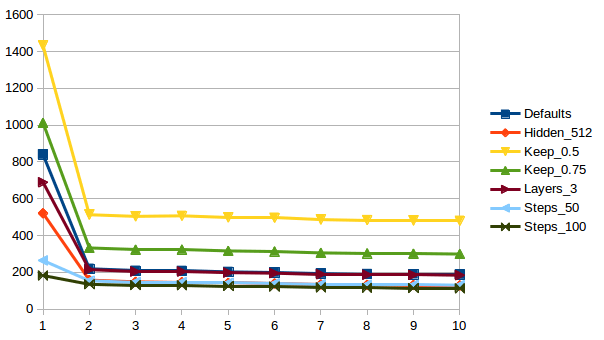
\includegraphics[width=0.75\textwidth]{epochs1.png}
    \caption{Test parameters over third epoch}
  \end{center}
\end{figure}


\begin{figure}[b]
  \begin{center}
    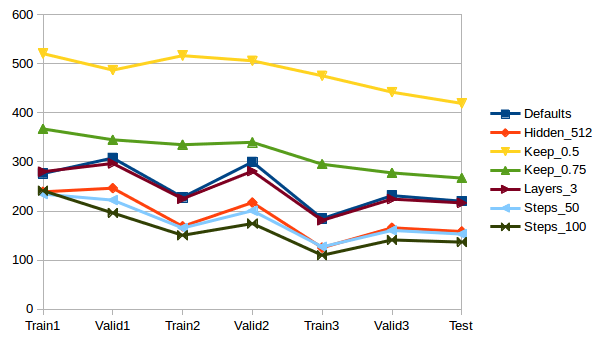
\includegraphics[width=0.75\textwidth] {train-valid-test1.png}
    \caption{Training, Validation, and Test Perplexity}
  \end{center}
\end{figure}

\clearpage

\section{Best Runs Combined}

Combining the three best attributes into a "combo" set of hyperparameters proved to have excellent results. The changes made to the default hyperparameters were:


Number of Layers: 3


Number of Steps: 100


Hidden Size: 512

\begin{figure}[H]
  \begin{center}
    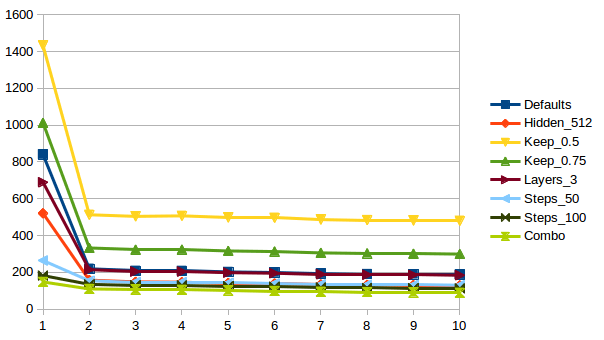
\includegraphics[width=0.75\textwidth] {epochs2.png}
    \caption{Combining Best hyperparameter changes}
  \end{center}
\end{figure}

\begin{figure}[H]
  \begin{center}
    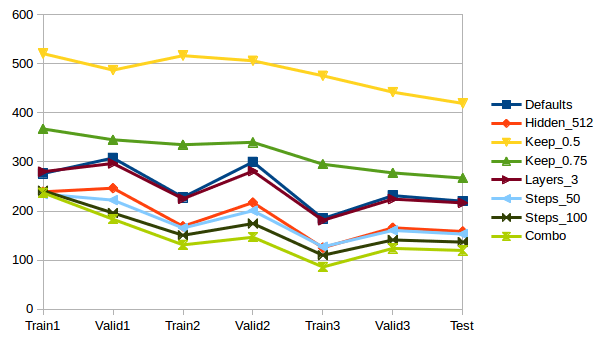
\includegraphics[width=0.75\textwidth] {train-valid-test2.png}
    \caption{Combining Best hyperparameter changes}
  \end{center}
\end{figure}

\clearpage

\section{Sentences}

\subsection{}

The default hyperparameters produced the following sentences:

Epoch 1: the company will be used in a [unk] test in a [unk] test in a [unk] test in a [unk] test

Epoch 2: the company said eos unk said it will be used in a [unk] test in a [unk] test in a [unk]

Epoch 3: the company said [eos] [unk] said it will be a [unk] in a [unk] [unk] in a [unk] [unk] in a

Test Perplexity: 220.851

-----

The sentences the default hyperparameters generated seemed to get stuck in a loop. Maybe from the limited number of epochs it was unable to capture significant information to make 20 words worth of text. The initial 3 to 5 words were more sentence-like, but quickly reverted to repetition.

\subsection{}

The combo hyperparameters produced the following sentences:

Epoch 1: the fed 's largest trade deficit [eos] the [unk] of the [unk] of the [unk] of the [unk] of the [unk]

Epoch 2: the largest trade index is n't expected to be in the u.s. market [eos] the fed has n't been able to

Epoch 3: the largest largest west german national league of the u.s. intelligence committee [eos] the fed has been [unk] with the u.s.

-----

The  combo hyperparameters which produced the lowest perplexity also produced the most comprehensible sentences. The first sentence had repetition like the default hyperparameters did, however the second and third epochs had longer strings of words which made logical sense.

\section{Mark/Trump Datasets}

\subsection{Mark Results}
Combo hyperparameters:


- Number of layers: 3


- Hidden units: 512


- Recurrent steps: 100


Running the default and combo hyperparameters on the Mark dataset gave the following results:



\begin{figure}[H]
  \begin{center}
    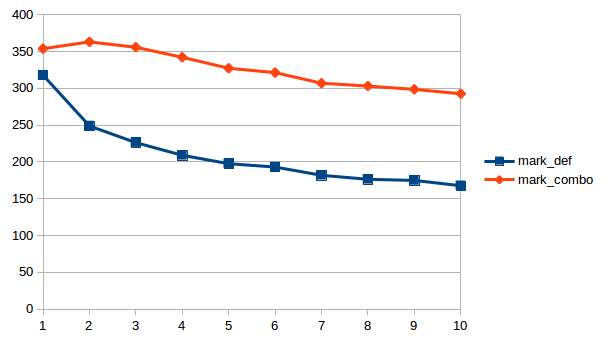
\includegraphics[width=0.75\textwidth] {mark1.png}
    \caption{Default and Combo hyperparameters on Mark Dataset; third epoch}
  \end{center}
\end{figure}

\begin{figure}[H]
  \begin{center}
    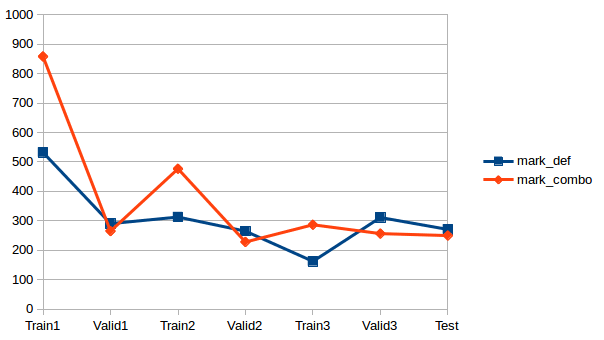
\includegraphics[width=0.75\textwidth] {mark2.png}
    \caption{Default and Combo hyperparameters on Mark Dataset; training, validation, and test}
  \end{center}
\end{figure}

We can see from the perplexity results in figures 5 and 6 that the combo hyperparameters proved moderately effective in decreasing perplexity compared to the default hyperparameters. Mostly the difference was noticeable in validation and test perplexity. It is interesting to note that the results aren't nearly as remarkable as the PTB dataset.

\subsection{Mark Sentences}
Default:


Epoch 1: the Lord had right the Lord will the Lord the Lord had right the Lord will the Lord the Lord had

Epoch 2: the right news the right will be right will be right will be right will be right will be right will

Epoch 3: the news and the Lord who will not been one who will not believe the good news the right news out

The default hyperparameters were able to capture some semblance of sentence structure or at least variation in words generated.

-----

Combo:


Epoch 1: the the the the the the the the the the the the the the the the the the the the the

Epoch 2: the the the the the the the the the the the the the the the the the the the the the

Epoch 3: the chief they will not the whole he will be the whole the whole they will not the whole he will

The combo hyperparameters seemed to get stuck early on. For 2 epochs the strongest association to "the" was "the" leading to an infinite loop. It was able to break out of this by epoch 3 and produce more variation, but is not very sentence-like. The very small vocabulary and dataset size could cause such effects on the generated output, as well as the diminished effect the combo hyperparameters had on the perplexity.

\subsection{Trump Results}

\begin{figure}[H]
  \begin{center}
    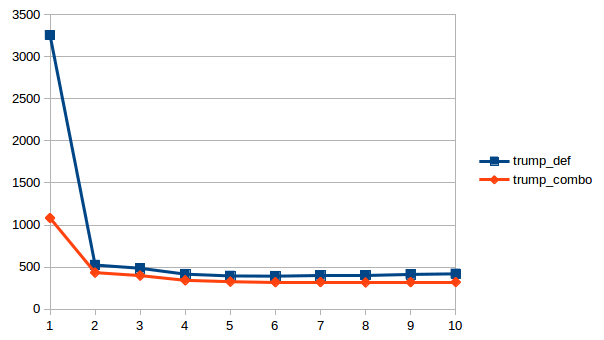
\includegraphics[width=0.75\textwidth] {trump1.png}
    \caption{Default and Combo hyperparameters on Trump Dataset; third epoch}
  \end{center}
\end{figure}

\begin{figure}[H]
  \begin{center}
    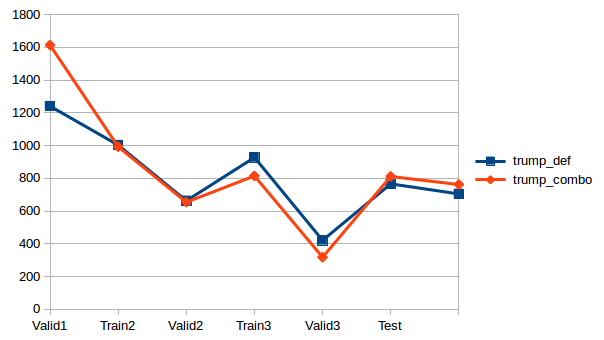
\includegraphics[width=0.75\textwidth] {trump2.png}
    \caption{Default and Combo hyperparameters on Trump Dataset; training, validation, and test}
  \end{center}
\end{figure}

Changing hyperparameters had even less of an effect on the Trump dataset. The vocabulary size for this dataset was more than triple the vocabulary size for PTB. Wheras the Mark dataset vocabulary was too small, this dataset had too large a vocabulary to form meaningful relationships between words. This, coupled with complexities related to twitter such as usernames, hashtags, etc, could have led to the  diminished effect of the combo hyperparameters compared to the previous datasets.

\subsection{Trump Sentences}
Default:


Epoch 1: the Obama is a great time of the Obama is a great time of the Obama is a great time of

Epoch 2: the @Yankees thing you can do well in the next debate. -- @MittRomney will be a great time to the debate

Epoch 3: the @Yankees game of the @Yankees game last night. <eos>I have to do well in the debate of the @Yankees game

The sentences generated by the default hyperparameters were repetitive and random. But they still read like proper Trump tweets.



Combo:


Epoch 1: the debate of the debate of the debate of the debate of the debate of the debate of the debate of

Epoch 2: the @Yankees in the world is a total in the debate of the next season of Obama to the debate of

Epoch 3: the most most years of the world in the world is the most important in the world in the debate he

The combo hyperparameters led to more structured sentences but, like in the Mark dataset, were initially more repetitive. 

\end{document}